
\documentclass[letterpaper,hide notes,xcolor={table,svgnames},pdftex,10pt]{beamer}
\def\showexamples{t}

\usecolortheme{crane}
\setbeamertemplate{navigation symbols}{}

\usetheme{MyPittsburgh}
\usepackage{hyperref}
\usepackage{graphicx,xspace}
\usepackage[normalem]{ulem}
\usepackage{multicol}
\usepackage{amsmath,amssymb,amsthm,graphicx,xspace}
\newcommand\SF[1]{$\bigstar$\footnote{SF: #1}}

\usepackage[sfdefault,lf]{carlito}
\usepackage[T1]{fontenc}
\usepackage[scaled]{beramono}
\usepackage{tikzpagenodes}
\newcommand{\Rplus}{\protect\hspace{-.1em}\protect\raisebox{.35ex}{\small{\small\textbf{+}}}}
\newcommand{\Cpp}{\mbox{C\Rplus\Rplus}\xspace}

\newcounter{tmpnumSlide}
\newcounter{tmpnumNote}

\newcommand\mnote[1]{%
	\addtocounter{tmpnumSlide}{1}
	\ifdefined\showcues {~\tiny\fbox{\arabic{tmpnumSlide}}}\fi
	\note{\setlength{\parskip}{1ex}\addtocounter{tmpnumNote}{1}\textbf{\Large \arabic{tmpnumNote}:} {#1\par}}}

\newcommand\mmnote[1]{\note{\setlength{\parskip}{1ex}#1\par}}


\newcommand\mquestion[2]{{~\color{red}\fbox{?}}\note{\setlength{\parskip}{1ex}\par{\Large \textbf{?}} #1} \note{\setlength{\parskip}{1ex}\par{\Large \textbf{A}} #2\par}\ifdefined \presentationonly \pause \fi}

\newcommand\blackboard[1]{%
	\ifdefined   \showblackboard
		{#1}
	\else {\begin{center} \fbox{\colorbox{blue!30}{%
						\begin{minipage}{.95\linewidth}%
							\hspace{\stretch{1}} Some space intentionally left blank; done at the blackboard.%
						\end{minipage}}}\end{center}}%
	\fi%
}

\usepackage{listings}
\lstset{%
	keywordstyle=\bfseries,
	aboveskip=15pt,
	belowskip=15pt,
	captionpos=b,
	identifierstyle=\ttfamily,
	frame=lines,
	numbers=left, basicstyle=\scriptsize, numberstyle=\tiny, stepnumber=0, numbersep=2pt}

\usepackage{siunitx}
\newcommand\sius[1]{\num[group-separator = {,}]{#1}\si{\micro\second}}
\newcommand\sims[1]{\num[group-separator = {,}]{#1}\si{\milli\second}}
\newcommand\sins[1]{\num[group-separator = {,}]{#1}\si{\nano\second}}
\sisetup{group-separator = {,}, group-digits = true}

%% -------------------- tikz --------------------
\usepackage{tikz}
\usetikzlibrary{positioning}
\usetikzlibrary{arrows,backgrounds,automata,decorations.shapes,decorations.pathmorphing,decorations.markings,decorations.text}

\tikzstyle{place}=[circle,draw=blue!50,fill=blue!20,thick, inner sep=0pt,minimum size=6mm]
\tikzstyle{transition}=[rectangle,draw=black!50,fill=black!20,thick, inner sep=0pt,minimum size=4mm]

\tikzstyle{block}=[rectangle,draw=black, thick, inner sep=5pt]
\tikzstyle{bullet}=[circle,draw=black, fill=black, thin, inner sep=2pt]

\tikzstyle{pre}=[<-,shorten <=1pt,>=stealth',semithick]
\tikzstyle{post}=[->,shorten >=1pt,>=stealth',semithick]
\tikzstyle{bi}=[<->,shorten >=1pt,shorten <=1pt, >=stealth',semithick]

\tikzstyle{mut}=[-,>=stealth',semithick]

\tikzstyle{treereset}=[dashed,->, shorten >=1pt,>=stealth',thin]

\usepackage{ifmtarg}
\usepackage{xifthen}
\makeatletter
% new counter to now which frame it is within the sequence
\newcounter{multiframecounter}
% initialize buffer for previously used frame title
\gdef\lastframetitle{\textit{undefined}}
% new environment for a multi-frame
\newenvironment{multiframe}[1][]{%
	\ifthenelse{\isempty{#1}}{%
		% if no frame title was set via optional parameter,
		% only increase sequence counter by 1
		\addtocounter{multiframecounter}{1}%
	}{%
		% new frame title has been provided, thus
		% reset sequence counter to 1 and buffer frame title for later use
		\setcounter{multiframecounter}{1}%
		\gdef\lastframetitle{#1}%
	}%
	% start conventional frame environment and
	% automatically set frame title followed by sequence counter
	\begin{frame}%
		\frametitle{\lastframetitle~{\normalfont(\arabic{multiframecounter})}}%
		}{%
	\end{frame}%
}
\makeatother

\makeatletter
\newdimen\tu@tmpa%
\newdimen\ydiffl%
\newdimen\xdiffl%
\newcommand\ydiff[2]{%
	\coordinate (tmpnamea) at (#1);%
	\coordinate (tmpnameb) at (#2);%
	\pgfextracty{\tu@tmpa}{\pgfpointanchor{tmpnamea}{center}}%
	\pgfextracty{\ydiffl}{\pgfpointanchor{tmpnameb}{center}}%
	\advance\ydiffl by -\tu@tmpa%
}
\newcommand\xdiff[2]{%
	\coordinate (tmpnamea) at (#1);%
	\coordinate (tmpnameb) at (#2);%
	\pgfextractx{\tu@tmpa}{\pgfpointanchor{tmpnamea}{center}}%
	\pgfextractx{\xdiffl}{\pgfpointanchor{tmpnameb}{center}}%
	\advance\xdiffl by -\tu@tmpa%
}
\makeatother
\newcommand{\copyrightbox}[3][r]{%
	\begin{tikzpicture}%
		\node[inner sep=0pt,minimum size=2em](ciimage){#2};
		\usefont{OT1}{phv}{n}{n}\fontsize{4}{4}\selectfont
		\ydiff{ciimage.south}{ciimage.north}
		\xdiff{ciimage.west}{ciimage.east}
		\ifthenelse{\equal{#1}{r}}{%
			\node[inner sep=0pt,right=1ex of ciimage.south east,anchor=north west,rotate=90]%
			{\raggedleft\color{black!50}\parbox{\the\ydiffl}{\raggedright{}#3}};%
		}{%
			\ifthenelse{\equal{#1}{l}}{%
				\node[inner sep=0pt,right=1ex of ciimage.south west,anchor=south west,rotate=90]%
				{\raggedleft\color{black!50}\parbox{\the\ydiffl}{\raggedright{}#3}};%
			}{%
				\node[inner sep=0pt,below=1ex of ciimage.south west,anchor=north west]%
				{\raggedleft\color{black!50}\parbox{\the\xdiffl}{\raggedright{}#3}};%
			}
		}
	\end{tikzpicture}
}


%% --------------------

%\usepackage[excludeor]{everyhook}
%\PushPreHook{par}{\setbox0=\lastbox\llap{MUH}}\box0}

%\vspace*{\stretch{1}

%\setbox0=\lastbox \llap{\textbullet\enskip}\box0}

\setlength{\parskip}{\fill}

\newcommand\noskips{\setlength{\parskip}{1ex}}
\newcommand\doskips{\setlength{\parskip}{\fill}}

\newcommand\xx{\par\vspace*{\stretch{1}}\par}
\newcommand\xxs{\par\vspace*{2ex}\par}
\newcommand\tuple[1]{\langle #1 \rangle}
\newcommand\code[1]{{\sf \footnotesize #1}}
\newcommand\ex[1]{\uline{Example:} \ifdefined \presentationonly \pause \fi
	\ifdefined\showexamples#1\xspace\else{\uline{\hspace*{2cm}}}\fi}

\newcommand\ceil[1]{\lceil #1 \rceil}


\AtBeginSection[]
{
	\begin{frame}
		\frametitle{Outline}
		\tableofcontents[currentsection]
	\end{frame}
}



\pgfdeclarelayer{edgelayer}
\pgfdeclarelayer{nodelayer}
\pgfsetlayers{edgelayer,nodelayer,main}

\tikzstyle{none}=[inner sep=0pt]
\tikzstyle{rn}=[circle,fill=Red,draw=Black,line width=0.8 pt]
\tikzstyle{gn}=[circle,fill=Lime,draw=Black,line width=0.8 pt]
\tikzstyle{yn}=[circle,fill=Yellow,draw=Black,line width=0.8 pt]
\tikzstyle{empty}=[circle,fill=White,draw=Black]
\tikzstyle{bw} = [rectangle, draw, fill=blue!20,
text width=4em, text centered, rounded corners, minimum height=2em]

\newcommand{\CcNote}[1]{% longname
	This work is licensed under the \textit{Creative Commons #1 3.0 License}.%
}
\newcommand{\CcImageBy}[1]{%
	\includegraphics[scale=#1]{creative_commons/cc_by_30.pdf}%
}
\newcommand{\CcImageSa}[1]{%
	\includegraphics[scale=#1]{creative_commons/cc_sa_30.pdf}%
}
\newcommand{\CcImageNc}[1]{%
	\includegraphics[scale=#1]{creative_commons/cc_nc_30.pdf}%
}
\newcommand{\CcGroupBySa}[2]{% zoom, gap
	\CcImageBy{#1}\hspace*{#2}\CcImageNc{#1}\hspace*{#2}\CcImageSa{#1}%
}
\newcommand{\CcLongnameByNcSa}{Attribution-NonCommercial-ShareAlike}

\newenvironment{changemargin}[1]{% 
	\begin{list}{}{% 
		\setlength{\topsep}{0pt}% 
		\setlength{\leftmargin}{#1}% 
		\setlength{\rightmargin}{1em}
		\setlength{\listparindent}{\parindent}% 
		\setlength{\itemindent}{\parindent}% 
		      \setlength{\parsep}{\parskip}% 
		      }% 
		\item[]}{\end{list}}




\title{Lecture 5 --- Processes in UNIX}

\author{Jeff Zarnett \\ \small \texttt{jzarnett@uwaterloo.ca}}
\institute{Department of Electrical and Computer Engineering \\
	University of Waterloo}
\date{\today}


\begin{document}

\begin{frame}
	\titlepage

\end{frame}

\begin{frame}
	\frametitle{The Process in UNIX}

	In UNIX a process may create other processes.

	The creating process is the parent; newly-created is the child.

	Every process has a parent, stretching back to \texttt{init}.

\end{frame}


\begin{frame}
	\frametitle{UNIX Process}
	Each process has a unique identifier in its process control block.

	This is the \texttt{pid} (process ID).

	For the most part, users will not need to know or think about the ID.

	Exception when trying to terminate one that's gotten stuck.\\
	\quad (\texttt{kill -9 24601}).

	The \texttt{init} process always gets a \texttt{pid} of 1.

	I don't recommend trying to kill \texttt{init}.

\end{frame}

\begin{frame}
	\frametitle{Linux Process Tree}

	\begin{center}
		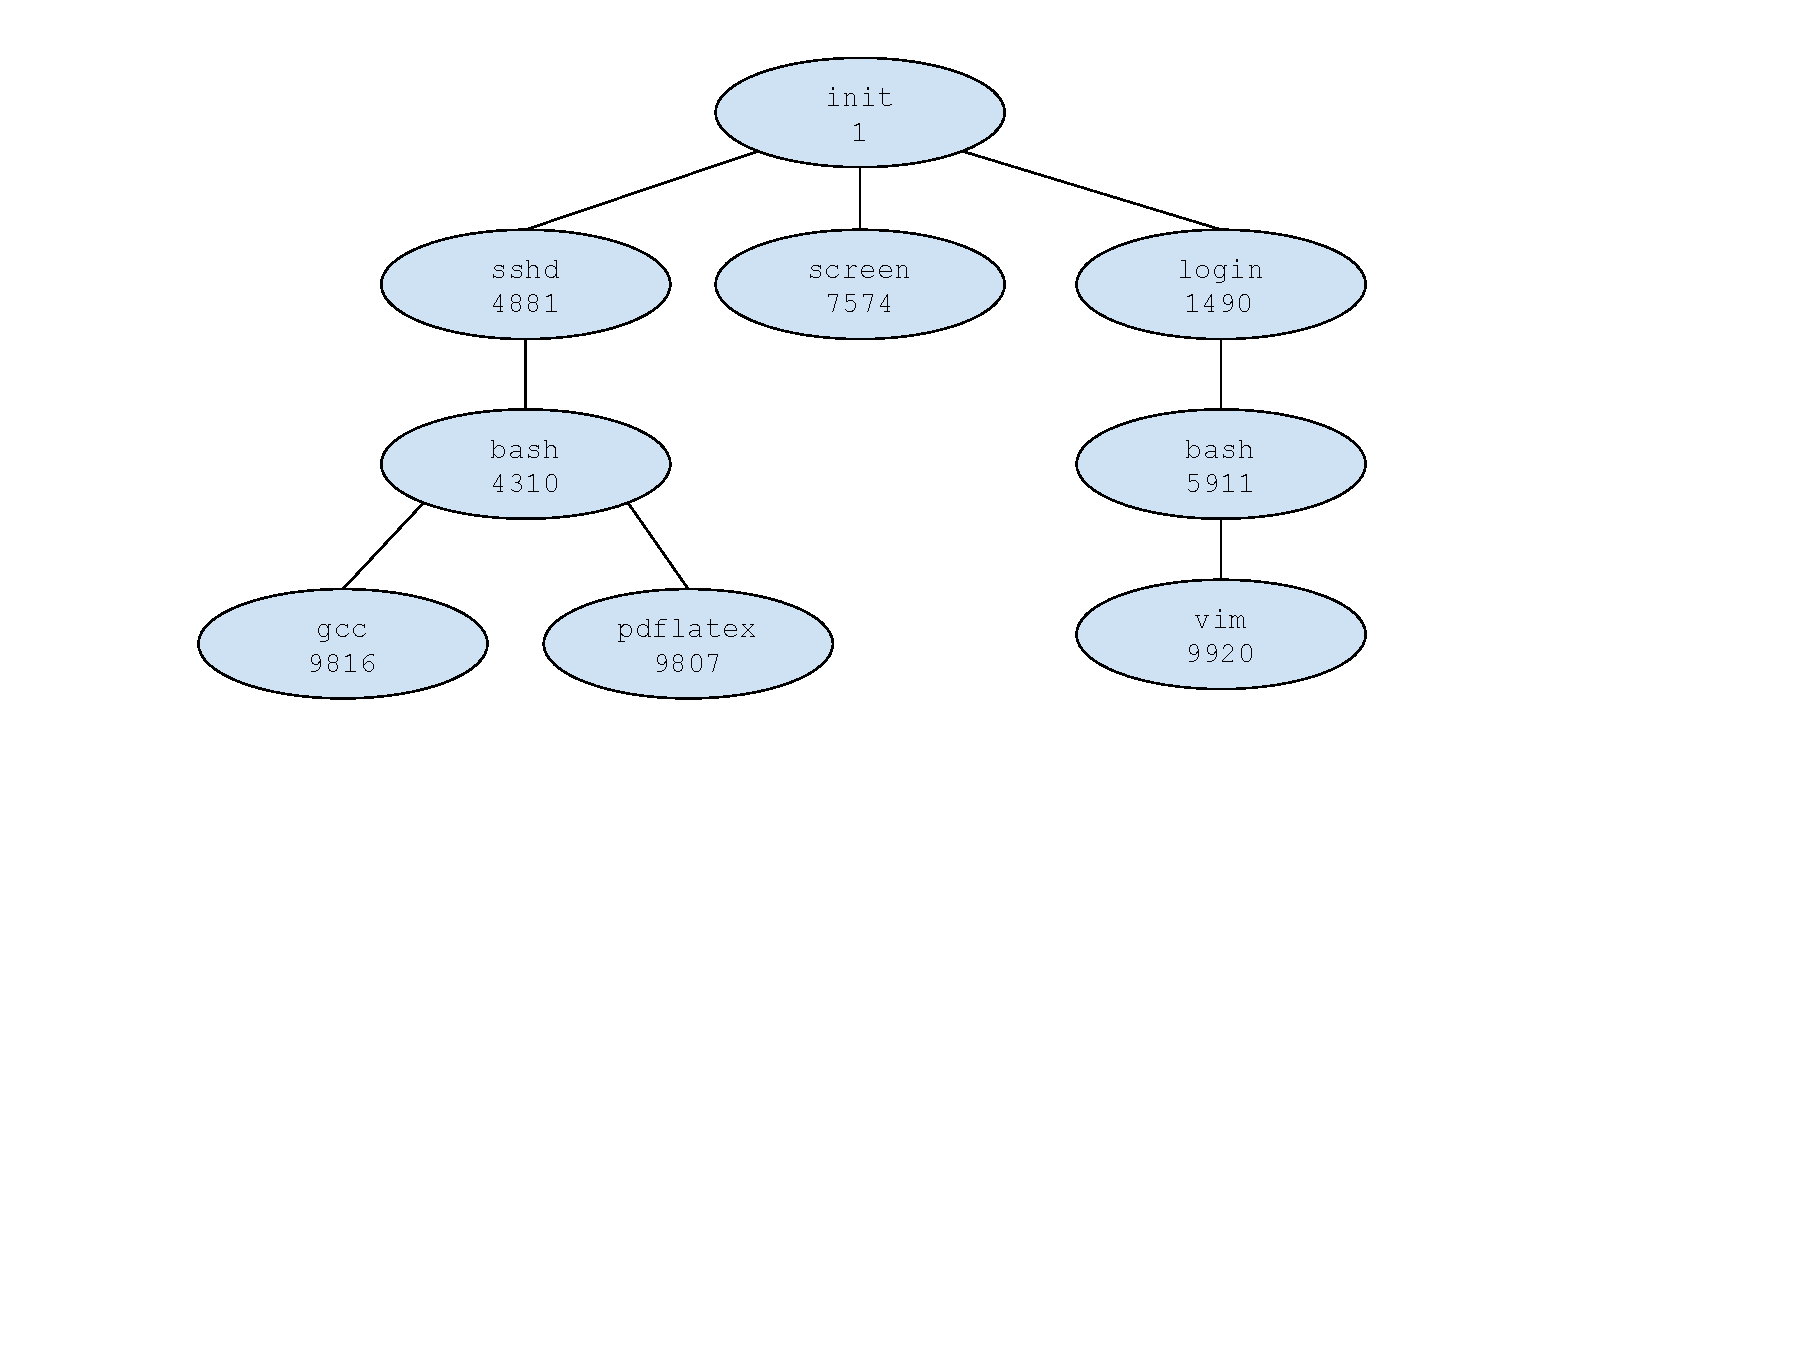
\includegraphics[width=\textwidth]{images/linux-process-tree.pdf}
	\end{center}

\end{frame}

\begin{frame}
	\frametitle{The \texttt{ps} Command}

	We can obtain a list of processes with \texttt{ps}.

	The diagram shows each user gets a \texttt{login} process.

	The shell (\texttt{bash}) is spawned from \texttt{login}.

\end{frame}

\begin{frame}
	\frametitle{Terminal Commands}

	When you issue a command, like \texttt{ls} or \texttt{top} (table of processes), the new process is created and the shell will \texttt{wait} on that process.

	It might finish on its own (e.g., \texttt{ls}).\\
	\quad Or wait for the user to tell it to exit (\texttt{top})

	When it does, control goes back to the shell.\\
	\quad You get presented with the prompt again (e.g., \texttt{jz@Loki:\~{}/\$}).

	Must I log in to the system in a second terminal window to run two things at a time?

	The answer is no, and there are two ways to get around it.

\end{frame}

\begin{frame}
	\frametitle{Run in the Background}

	Option 1: tell the shell we want the task to run in the background.

	To do that, add to the command the \texttt{\&} symbol:

	\texttt{gcc fork.c \&}

	Control returns almost immediately to the shell.\\
	\quad It is not waiting for \texttt{gcc} to finish.

\end{frame}

\begin{frame}
	\frametitle{Run in the Background}

	You may see some output like \texttt{[1] 34429}.

	This is the shell saying: child has been created; it has process ID 34429.

	When the process is finished, there is another update:

	\texttt{[1]+  Done                    gcc fork.c}

\end{frame}

\begin{frame}
	\frametitle{Run in the Background}

	Notably, any console output that the \texttt{gcc} command would generate will still appear on the console where the background task was created.

	Maybe you want that but maybe you want to put the output in a log file, with a command like \texttt{cat fork.c > logfile.txt \&}.

	(Telling \texttt{gcc} to be silent is a somewhat more complex operation.)

\end{frame}

\begin{frame}
	\frametitle{Example of the \&}

	A common example of a command I use involving the \texttt{\&}:\\
	\texttt{ sudo service xyz start \& }

	This will (with super user permissions) start up the service \texttt{xyz}.

	It returns control to the console so I don't have to wait.

	Next: \texttt{tail -f /var/log/xyz/console.log}

	Watch the console log of the \texttt{xyz} service as it starts up.

\end{frame}

\begin{frame}
	\frametitle{Option Two: \texttt{screen}}

	The other alternative is the \texttt{screen} command.

	While having something run in the background is nice, it does not work for interactive processes.

	Example: text editing with \texttt{vi} and want to read e-mail with \texttt{pine}.

	Could be done by saving and closing \texttt{vi}.

	Or, start them in \texttt{screen} and switch between them.

\end{frame}

\begin{frame}
	\frametitle{Using \texttt{screen}}
	Instead of just opening \texttt{vi fork.c} I can issue the command \texttt{screen vi fork.c} and this spawns \texttt{screen} and takes me right to editing the file.

	The key difference is that I can ``detach'' from this screen and go back to the command line.

	If I log out, \texttt{screen} keeps running with the \texttt{vi} inside it.

	If I have multiple screens running, I can just ``reattach'' to the one I want.

\end{frame}

\begin{frame}
	\frametitle{UNIX Workflow}

	Parent spawns the child process with the \texttt{fork} system call.

	If waiting for the child process to finish, \texttt{wait}.\\
	\quad Alternatively, carry on.

	When the child process is finished, it returns a value with \texttt{exit}

	The parent gets this as the return value of \texttt{wait} and may proceed.
\end{frame}

\begin{frame}
	\frametitle{About \texttt{fork}}

	Note: \texttt{fork} creates a new process as a copy of itself.

	\begin{center}
		
\includegraphics[width=0.4\textwidth]{images/spiderman-2.jpg}
	\end{center}

	Both parent and child continue after that statement.

	The call \texttt{fork} can return a value:\\
	\quad A negative value means the fork failed.\\
	\quad A zero value means this process is the child.\\
	\quad A positive value: this is the parent; the value is the child \texttt{pid}.

\end{frame}

\begin{frame}
	\frametitle{After the \texttt{fork}, the \texttt{exec}}


	After the \texttt{fork}, one of the processes may use the \texttt{exec} system call.

	This will replace its memory space with a new program.

	There's no rule that says this must happen\\
	\quad a child can continue to be a clone of its parent if it wishes.

	The \texttt{exec} invocation loads a binary file into memory \& starts execution.

	At this point, the programs can go their separate ways.

	Or the parent might want to wait for the child to finish.


\end{frame}

\begin{frame}[fragile]
	\frametitle{Putting it Together}

	{\scriptsize
		\begin{lstlisting}[language=C]
int main( int argc, char** argv ) {
  pid_t pid;
  int childStatus;

  /* fork a child process */
  pid = fork();
  
  if (pid < 0) { 
    /* error occurred */ 
    fprintf(stderr, "Fork Failed"); 
    return 1;
  
 } else if (pid == 0) {    
    /* child process */
    execlp("/bin/ls","ls",NULL);
    
  } else {    
    /* parent process */
    /* parent will wait for the child to complete */
    wait(&childStatus);
    printf("Child Complete with status: %i \n", childStatus);
    
  }
    
  return 0;
}
\end{lstlisting}
	}

\end{frame}

\begin{frame}[fragile]
	\frametitle{Code Output}

	Thus, the output is:
	\begin{verbatim}
jz@Freyja:~/fork$ ./fork 
fork   fork.c
Child Complete with status: 0
jz@Freyja:~/fork$ 
\end{verbatim}


\end{frame}

\begin{frame}
	\frametitle{Fork Visually}

	Or, to represent this visually:

	\begin{center}
		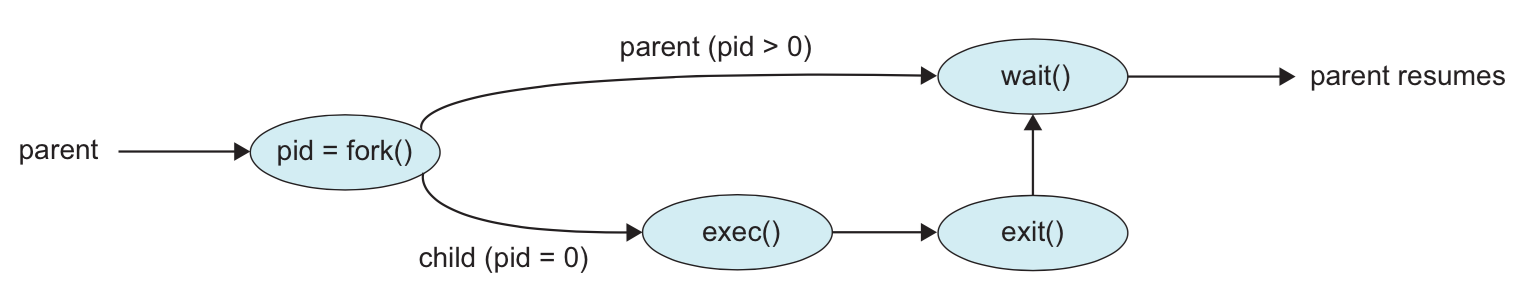
\includegraphics[width=\textwidth]{images/fork-syscall.png}
	\end{center}

\end{frame}

\begin{frame}
	\frametitle{Termination?}

	What about termination?

	On the assumption that the process is terminating normally and not being killed, the system call for that is \texttt{exit}.

	If the program itself has no explicit call to \texttt{exit}, the \texttt{return} statement at the end of \texttt{main} will have the same effect.

	Let us modify that code above to fork off a child process that will exit ``abnormally'' with an exit code of 1.

	The \texttt{wait} function also returns the process ID of the child.

	This is so that the parent can identify which of its children has terminated, though it is not used in this example.

\end{frame}

\begin{frame}
	\frametitle{After the \texttt{fork}}

	Afterwards, the system will need to choose which process is going to run:

	\begin{enumerate}
		\item The parent process. The child is in the ready to run state.
		\item The child process. The parent is in the ready to run state.
		\item Another process. Both parent and child are in the ready to run state.
	\end{enumerate}

\end{frame}


\begin{frame}
	\frametitle{Fork Design Problem}

	There is a task that can be split into parts 'A' and 'B'.

	Use \texttt{fork()} to create a child process.

	The child process should call function \texttt{execute\_B()} and return the result to the parent.

	The parent process should call \texttt{execute\_A()} and collect its result.

	The parent should then collect the result of the child using \texttt{wait()} and then produce the console output.

\end{frame}

\begin{frame}
	\frametitle{Fork Design Problem}
	If no errors occurred, \texttt{main} should return 0; otherwise it should return -1.

	If an error occurs, it should be reported to the console including the error number (e.g., ``Error 7 Occurred.'').

	If more than one error occurs, report both errors.

	If both functions return zero, it means all is well and the program should print ``Completed.'' to the console.

\end{frame}


\begin{frame}[fragile]
	\frametitle{Fork Design Solution}
	\begin{lstlisting}[language=C]
int main( int argc, char** argv ) {
  int child_result;
  int parent_result;

  pid_t pid = fork();
  if ( pid < 0 ) { /* Fork Failed */
    return -1;
  } else if ( pid == 0 ) { /* Child */
    return execute_B();
  } else { /* Parent */ 
    parent_result = execute_A();
    wait( &child_result );
  }
  
  if ( child_result == 0 && parent_result == 0 ) {
    printf( "Completed.\n" );
    return 0;
  }
  
  if ( child_result != 0 ) {
    printf( "Error %d Occurred.\n", child_result);
  }
  if ( parent_result != 0 ) {
    printf( "Error %d Occurred.\n", parent_result);
  }
  return -1;
}
\end{lstlisting}
\end{frame}

\begin{frame}
	\frametitle{Apr\`{e}s \texttt{fork}, le d\'{e}luge}

	A short digression on a denial of service attack: the ``fork bomb''.

	The idea is to call \texttt{fork} repeatedly.

	Keep doing this until the system crashes (or no work can get done).

	Exponential growth ($2^n$) processes after $n$ calls.

\end{frame}


\begin{frame}
	\frametitle{Fork Bomb}

	\begin{center}
		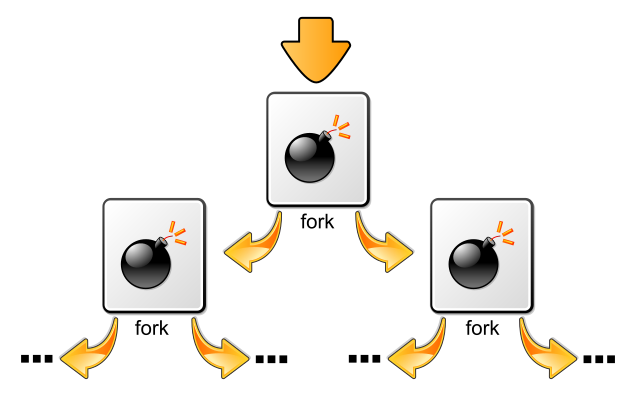
\includegraphics[width=\textwidth]{images/forkbomb.png}
	\end{center}
	\hfill Image Credit: Wikipedia user Dake

\end{frame}


\begin{frame}
	\frametitle{Apr\`{e}s \texttt{fork}, le d\'{e}luge}
	A system can be configured to defend against this.

	1. Limit total number of processes per user.

	2. Limit rate of process spawning.

	Note: do not attempt this on University computers!

\end{frame}


\begin{frame}
	\frametitle{Signals}

	UNIX systems use signals to indicate events (e.g., the \texttt{Ctrl-C} on the console)

	Signals also are things like exceptions (division by zero, segmentation fault).

	It is \textit{synchronous} if the signal occurs as a result of the program execution (e.g., dividing by zero);

	It is \textit{asynchronous} if it comes from outside the process (e.g., the user pressing \texttt{Ctrl-C} or one process or thread sending a signal to another).

	Signals are, in the end, interrupts with a certain integer ID.


\end{frame}


\begin{frame}
	\frametitle{Gondor Calls For Aid}

	\begin{center}
		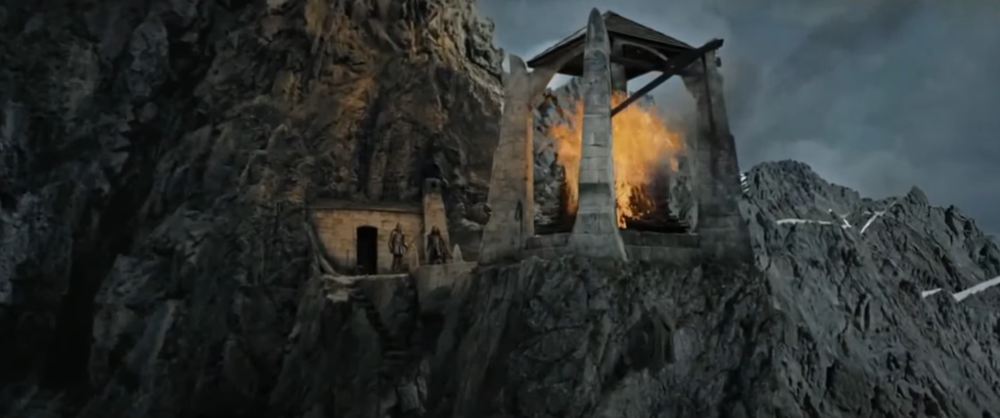
\includegraphics[width=\textwidth]{images/beacon_gondor.png}
	\end{center}

\end{frame}



\begin{frame}
	\frametitle{Signals}

	By default, the kernel will handle any signal that is sent to a process with the default handler.

	The behaviour of the default handler may be to ignore the signal, but some signals (segmentation fault) will result in termination of the process.


\end{frame}


\begin{frame}
	\frametitle{POSIX Signals}

	Here are some of the many signals described in the POSIX.1-1990 standard:

	{\scriptsize
	\begin{center}
		\begin{tabular}{l|l|l|l}
			\textbf{Signal}  & \textbf{Comment}                              & \textbf{Value} & \textbf{Default Action}            \\ \hline
			\texttt{SIGHUP}  & Hangup detected                               & 1              & Terminate process                  \\
			\texttt{SIGINT}  & Keyboard interrupt (\texttt{Ctrl-C})          & 2              & Terminate process                  \\
			\texttt{SIGQUIT} & Quit from keyboard                            & 3              & Terminate process, dump debug info \\
			\texttt{SIGILL}  & Illegal instruction                           & 4              & Terminate process, dump debug info \\
			\texttt{SIGKILL} & Kill signal                                   & 9              & Terminate process                  \\
			\texttt{SIGSEGV} & Segmentation fault (invalid memory reference) & 11             & Terminate process, dump debug info \\
			\texttt{SIGTERM} & Termination signal                            & 15             & Terminate process                  \\
			\texttt{SIGCHLD} & Child stopped or terminated                   & 20,17,18       & Ignore                             \\
			\texttt{SIGCONT} & Continue if stopped                           & 19,18,25       & Continue the process if stopped    \\
			\texttt{SIGSTOP} & Stop process                                  & 18,20,24       & Stop process                       \\
		\end{tabular}
	\end{center}
	}

\end{frame}


\begin{frame}
	\frametitle{Handling Signals}

	A process may inform the OS it is prepared to handle a signal itself.

	Example: doing some cleanup when \texttt{Ctrl-C} is received instead of just dying.

	In any event, a signal needs to be handled, even if the handling is to ignore it.

	The signals \texttt{SIGKILL} and \texttt{SIGSTOP} cannot be caught, blocked, or ignored.


\end{frame}


\begin{frame}
	\frametitle{Command-Line Signals}

	On the command line: to send a signal, \texttt{kill} followed by a process ID.

	Normally a command like \texttt{kill 24601} will send \texttt{SIGHUP} to a process.

	This will, by default, kill the process.\\
	\quad The process has an opportunity to clean things up if it wants to.

	If the process is still stuck, you can ``force'' kill the process with \texttt{SIGKILL}:\\\ \quad \texttt{kill -9 24601}.

	The \texttt{-9} parameter sends signal 9 (\texttt{SIGKILL}) rather than the default 1 (\texttt{SIGHUP}).

	Some users are eager to jump to \texttt{kill -9} whenever a process is stuck...
\end{frame}






\end{document}

